% Cover letter using letter.sty

\documentclass[11pt]{letter} % Uses 10pt
\usepackage{graphicx,subfigure}
\usepackage{float}
\usepackage{caption}
\captionsetup{labelsep=space}

\renewcommand*{\figureformat}{\figurename~\thefigure}

\restylefloat{figure}
%Use \documentstyle[newcent]{letter} for New Century Schoolbook postscript font
% the following commands control the margins:
\topmargin=-1.2in    % Make letterhead start about 1 inch from top of page 
\textheight=14in  % text height can be bigger for a longer letter
\oddsidemargin=0pt % leftmargin is 1 inch
\textwidth=6.5in   % textwidth of 6.5in leaves 1 inch for right margin
\textheight 255mm


\begin{document}\pagenumbering{gobble}




\begin{flushleft}
{\large\bf Eamon O'Gorman - Research Interests and Future Plans}
\end{flushleft}
\medskip\hrule height 1pt
\begin{flushright}


\end{flushright} 
%\vfill % forces letterhead to top of page
\begin{center}
\textbf{Research Interests}
\end{center}\\
My research interests to date have focused on understanding the atmospheric properties of non-dusty late K and early M spectral type red giants and red supergiants (RSGs). These stars have substantial mass-loss rates yet the mechanisms which drives this large mass-loss are unknown and remain one of the great unsolved problems in modern stellar astrophysics. There is insufficient atomic, molecular, or dust opacity to drive a radiation-driven outflow and acoustic/pulsation models cannot drive the observed mass-loss rates. UV and optical observations reveal an absence of significant hot wind plasma, and the winds are thus too cool to be Parker-type thermally-driven flows. Magnetic fields are most likely involved in the mass-loss process, although current magnetic models are also unable to explain spectral diagnostics and spatially resolved radio continuum observations. Traditionally, observations of evolved stars have provided only limited disk-averaged information about the outflow environments of these stars, making it difficult to infer the wind properties. My primary research to date has focused on using the latest suite of millimeter and centimeter interferometers to provide essential spatial information on these outflow environments, to gain a better understanding of the entire mass-loss process.

Part of my research has focused on understanding the complex circumstellar environment of the enigmatic M supergiant Betelgeuse. Betelgeuse is one of the few nearby RSGs that can be studied in great detail across most of the electromagnetic spectrum. The extended atmosphere of this oxygen-rich RSG provides an ideal testbed for studying the poorly understood processes that drive mass-loss from K and M supergiants. Betelgeuse has undergone at least two distinct phases of mass-loss in its recent past. However, previous single dish millimeter observations were only able to detect one component of the outflow, while the spatial extent of both components were entirely unknown. Using multiple array configurations of the CARMA millimeter interferometer, we successfully imaged the CO($J = 2 - 1$) emission line at sub-arcsecond resolution, and for the first time were able to find the spatial extent of both outflow components, allowing their ages to be calculated (O'Gorman et al., 2012, \textit{AJ}). We found both flow components to be inhomogeneous, far from the existing spherically symmetric models of its circumstellar environment, indicating a chaotic mass-loss loss process. We also observed  the CO($J = 3 - 2$) emission line with the SMA millimeter interferometer and we found that both emission lines probed similar structure in the circumstellar environment (O'Gorman, 2013, \textit{Thesis}). 

The wind acceleration region is where most of the momentum and heat which drive the mass-loss in RSGs is deposited. Thermal millimeter and centimeter continuum emission directly sample this region which extends out to only a few $R_{\star}$. I have been heavily involved in a collaboration which has used e-MERLIN to image the thermal continuum emission from this inner region of Betelgeuse's atmosphere at 6\,cm (Richards et al., 2013). We have discovered two ``chromospheric hotspots'' (Figure 1, \textit{left}) separated by $4\,R_{\star}$, hidden just beyond the spatial resolution of the VLA at 6\,cm. Using the astrometric solution of Harper et al. (2008), the brighter hotspot ($T_{e} > 5400$\,K) is $\sim 3.5\,R_{\star}$ from the photosphere (O'Gorman, 2013, \textit{Thesis}). Inspired by this new discovery, I have analyzed multi-wavelength, multi-epoch, centimeter VLA data which contains the Pie Town VLBA antenna, to look for signatures of these hotspots. At the highest available frequencies, these data have even superior spatial resolution than e-MERLIN (at 6\,cm).  In Figure 1 (right) a preliminary map at 0.7\,cm is presented, and exciting evidence of at least two features separated by only $2\,R_{\star}$ is shown. These features may be generated by  giant photospheric convective cells, although it is unlikely that convection alone could be accountable for the hotspots seen with e-MERLIN (O'Gorman, 2014, \textit{In prep}).

We have recently used the JVLA to observe two non-dusty, non-pulsating, K spectral-type red giants at multiple radio wavelengths ($0.7 - 20$\,cm) (O'Gorman et al., 2013, \textit{AJ}). Such stars are feeble emitters at these wavelengths however, and previous observations provided only a small number of modest S/N measurements, slowly accumulated over three decades. Our observations of each star were carried out over just a few days, so that we obtained an essentially consistent snapshot of the different stellar atmospheric layers sampled at different wavelengths. We found that our observations were in disagreement with the existing semi-empirical atmospheric models for these stars, which were based only on UV diagnostics. We also found evidence for a rapidly cooling stellar wind for one of the targets which allowed us to develop a new semi-empirical wind model for the star. This model was then used as the basis to compute a thermal energy balance of the star's outflow by investigating the various heating (e.g., dissipation of Alfv\'en waves) and cooling processes (e.g., adiabatic expansion) that control its thermal structure (O'Gorman, 2013, \textit{Thesis}). 

\begin{figure}[!t]
\centering 
\mbox{
          \includegraphics[trim=27pt 90pt 40pt 90pt,clip,angle=90,width=8cm,height=7cm]{/home/eamon/jobs/naasc/plan/fig1.ps}
          \includegraphics[trim=110pt 505pt 140pt 20pt,clip,width=9.5cm,height=7.0cm]{/home/eamon/jobs/asiaa/plan/test2.ps}
          }
\caption{ {\small  \textbf{Figure 1.} \textit{Left:} e-MERLIN 6\,cm image of Betelgeuse showing the two ``chromospheric hotspots''. The red filled circle marks the expected photospheric position. \textit{Right:} VLA + Pie Town 0.7\,cm image of Betelgeuse's inner asymmetric atmosphere. The presence of giant photospheric convective cells can account for the asymmetries in the 0.7\,cm image, but cannot account for the hotspot at $\sim 3.5\,R_{\star}$ in the 6\,cm image.}}
\end{figure}

\begin{center}
\textbf{Future Plans}
\end{center}\\
The latest suite of radio interferometers such as ALMA, the JVLA, and e-MERLIN now have the capability of providing sensitive spatially resolved millimeter and centimeter observations of the atmospheres of the closest RSGs and red giants. As a postdoctoral researcher, I plan to carry out millimeter and centimeter observations of evolved stellar atmospheres which will contribute exciting new insights into the currently unknown mass-loss process in these stars. 

\textbf{Red Supergiants:}\\
I am part of a collaboration that has been awarded ALMA cycle 1 time (PI: P. Kervella) which will trace CO($J=6-5$) emission around Betelgeuse at a resolution 10 times higher (i.e., $\sim 0.1''$) than we achieved with the CARMA interferometer (discussed previously). Such observations will provide a detailed picture into the dynamics of the inner atmosphere of M supergiants. There has been much debate about the role dust plays in the mass-loss from RSGs and these observations will also be capable of imaging any dust which may lie just beyond $\sim 2.5\,R_{\star}$ of Betelgeuse, a relatively non-dusty M supergiant. These observations may be carried over to Cycle 2 if our project is not fully observed during Cycle 1 (i.e., by the end of May 2014). My past experience with analyzing millimeter interferometric data will be of great importance to this project and working with the first ALMA observations of a RSG may be my first project as a postdoctoral researcher. In the near future, ALMA should have sufficient spatial resolution ($\sim 50$ mas) at multiple frequencies to spatially resolve the free-free thermal emission from Belelgeuse and Antares (the two closest M supergiants). I envisage using ALMA at multiple frequencies to directly determine the temperature profiles of the  innermost atmospheres ($<2\,R_{\star}$) of these stars. Such measurements have previously been carried out by Lim et al., (1998) at longer wavelengths with the VLA and have probed the temperature between $2 < \,R_{\star} < 5$. However, observations at ALMA frequencies will probe the crucial innermost atmosphere where much of the energy that goes into driving the wind is deposited, and will confront existing models along with searching for evidence of the giant convection cells and the ``chromospheric hotspots'' seen at longer wavelengths (i.e., with the VLA and e-MERLIN respectively).

Our recent findings with the very long baseline interferometer, e-MERLIN, raise more questions about the mass-loss process in M supergiants than answers. What mass-loss process could cause such chromospheric hotspots on such large scales and on what time scales do they evolve? Multi-wavelength high spatial resolution monitoring of Betelgeuse with e-MERLIN is required to solve this puzzling evidence and this project will be one of my immediate priorities. The next call for e-MERLIN proposals is in spring 2014 and I plan to propose to observe Betelgeuse at both 6\,cm (C band) and 1.3\,cm (K band) for at least two epochs during this call. This multi-epoch multi-wavelength data will provide insights into the time scales on which the chromospheric hotspots evolve and may also be capable of spatially resolving them allowing their size and temperature to be directly determined. I also plan to apply for JVLA A-configuration time in August 2014 to observe Betelgeuse again at 6\,cm and 1.3\,cm with the intention of combining these data with data from e-MERLIN. Such data will produce the highest spatial resolution radio image ever of the thermal emission from any star other than our Sun. 

\textbf{Red Giants:}\\
The atmospheric properties of non-dusty red giant stars are still poorly understood and this ultimately leads to a lack of understanding into the mechanism by which they lose mass. These stars generally have smaller angular diameters than the nearest RSGs and currently cannot be spatially resolved at radio wavelengths; although ALMA will eventually change this. We have recently obtained multi-frequency millimeter thermal continuum observations of a sample of red giants (PI: E. O'Gorman, ID: C1038) with the CARMA interferometer, which I intend to reduce in my first year as a postdoctoral researcher. The intention is to combine these spatially unresolved data sets with our published JVLA data.  These combined data sets will then span over 4 orders of magnitudes of continuum optical depth probing many different layers of the star's atmosphere. These data sets can then be used to develop semi-empirical atmospheric models using our non-LTE hydrogen ionization code which solves the equation of radiative transfer by including advection in the rate equations. The ultimate goal will be to use these atmospheric models to calculate what is heating the winds of these stars, in turn providing insights into the unknown mass-loss mechanism. 

\textbf{Other Interests:}\\
My interests in astrophysics are wide and varied and I am very much interested in starting new collaborations where I could utilize my experience in millimeter and centimeter interferometry in other areas of astrophysics. An example of this is my ongoing project to detect radio emission from $\beta$ Gem b, an exoplanet orbiting the closet red giant, Pollux (PI: E. O’Gorman, ID: 24 013). Previous searches for exoplanet radio emission have focused on close orbiting planets, the so-called \textit{hot Jupiters}. Our target is further away from its host star and free from tidal locking, which may reduce the internal magnetic field of the hot Jupiters, thus reducing the strength of the radio emission. We expect the relatively large mass-loss of the host red giant to be a key driver in detecting this emission. We are currently using the GMRT to search for this emission at 150\,MHz. In June 2013, we obtained our first data set from the GMRT and we have just recently (22 November, 2013) obtained more data from the GMRT of this interesting system. I plan to carry out further observations of this interesting planetary system at lower frequencies and higher sensitivity with LOFAR as a postdoctoral researcher.

\end{flushright}
\end{document}






